\documentclass[12pt]{article}
\pagenumbering{gobble}
\linespread{1.1}

\usepackage{amsfonts}
\usepackage{amsmath}
\usepackage{amssymb}
\usepackage{array}
\usepackage{fancyhdr}
\usepackage{mathrsfs}
\usepackage{mathtools}
\usepackage{parskip}
\usepackage{textcomp}
\usepackage[margin=1in,headheight=1in]{geometry}

\usepackage{tikz}
\usetikzlibrary{arrows.meta}
\usetikzlibrary{calc}
\usetikzlibrary{shapes.geometric}

\newcommand{\contradiction}{
    \ensuremath{{\Rightarrow\mspace{-2mu}\Leftarrow}}
}

% bracket commands
\newcommand{\angleb}[1]{\left\langle#1\right\rangle} % <>
\newcommand{\vertb}[1]{\left\vert#1\right\vert}      % ||
\newcommand{\bracks}[1]{\left[#1\right]}             % []
\newcommand{\braces}[1]{\left\{#1\right\}}           % {}
\newcommand{\parens}[1]{\left(#1\right)}             % ()

% set aliases
\newcommand{\N}{\mathbb{N}}
\newcommand{\Z}{\mathbb{Z}}
\newcommand{\Q}{\mathbb{Q}}
\newcommand{\R}{\mathbb{R}}

\newcommand{\derv}[2]{\dfrac{d#1}{d#2}}
\newcommand{\e}{\varepsilon}
\newcommand{\di}{\,/\,}

\newcommand{\lm}[1]{\displaystyle\lim_{#1}}

\begin{document}
\pagestyle{fancy}
\fancyhead{}
\fancyhead[L]{Alex Agruso}
\fancyhead[R]{Topology Writing 9}

\normalsize

\begin{itemize}
    \item [a.)] In the metric space $(\R^2,d_{std})$, $\text{Ball}(0,1)$ looks like

    \begin{center}
        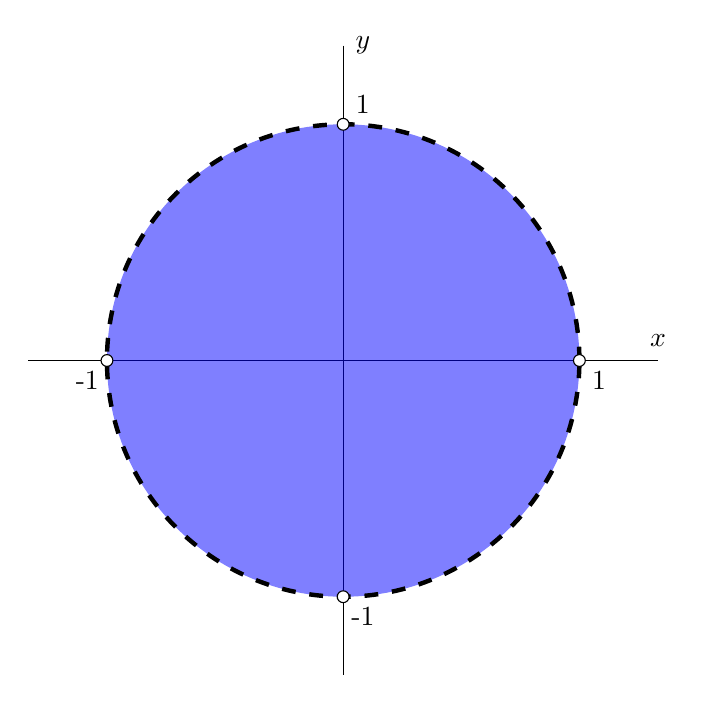
\begin{tikzpicture}
            \draw (-4,0) -- (4,0);
            \node at (4,0.25) {$x$};

            \draw (0,4) -- (0,-4);
            \node at (0.25,4) {$y$};

            \draw[ultra thick,dash=on 5pt off 5pt phase 10pt,fill=blue,fill opacity=0.5] (0,0) circle (3);

            \draw[fill=white] (-3,0) circle (0.075);
            \node at (-3.25,-0.25) {-1};

            \draw[fill=white] (3,0) circle (0.075);
            \node at (3.25,-0.25) {1};

            \draw[fill=white] (0,3) circle (0.075);
            \node at (0.25,3.25) {1};

            \draw[fill=white] (0,-3) circle (0.075);
            \node at (0.25,-3.25) {-1};
        \end{tikzpicture}
    \end{center}

    \item [b.)] In the metric space $(\R^2,d_{l^\infty})$, $\text{Ball}(0,1)$ looks like

    \begin{center}
        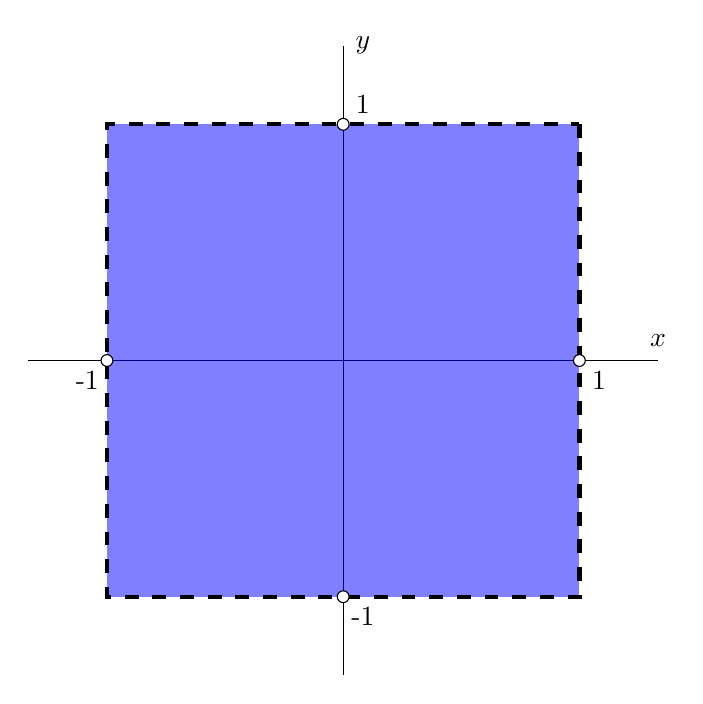
\begin{tikzpicture}
            \draw (-4,0) -- (4,0);
            \node at (4,0.25) {$x$};

            \draw (0,4) -- (0,-4);
            \node at (0.25,4) {$y$};

            % \filldraw [thick, fill=red, even odd rule] (0,0) coordinate (Square) -- ++(0,6) -- ++(4,0) -- ++(0,-4) -- cycle;
            \filldraw [ultra thick,dash=on 5pt off 5pt phase 10pt,fill=blue,fill opacity=0.5] (3,3) -- (3,-3) -- (-3,-3) -- (-3,3) -- cycle;

            \draw[fill=white] (-3,0) circle (0.075);
            \node at (-3.25,-0.25) {-1};

            \draw[fill=white] (3,0) circle (0.075);
            \node at (3.25,-0.25) {1};

            \draw[fill=white] (0,3) circle (0.075);
            \node at (0.25,3.25) {1};

            \draw[fill=white] (0,-3) circle (0.075);
            \node at (0.25,-3.25) {-1};
        \end{tikzpicture}
    \end{center}

    \pagebreak
    \item [c.)] In the metric space $(\R^2,d_{taxi})$, $\text{Ball}(0,1)$ looks like

    \begin{center}
        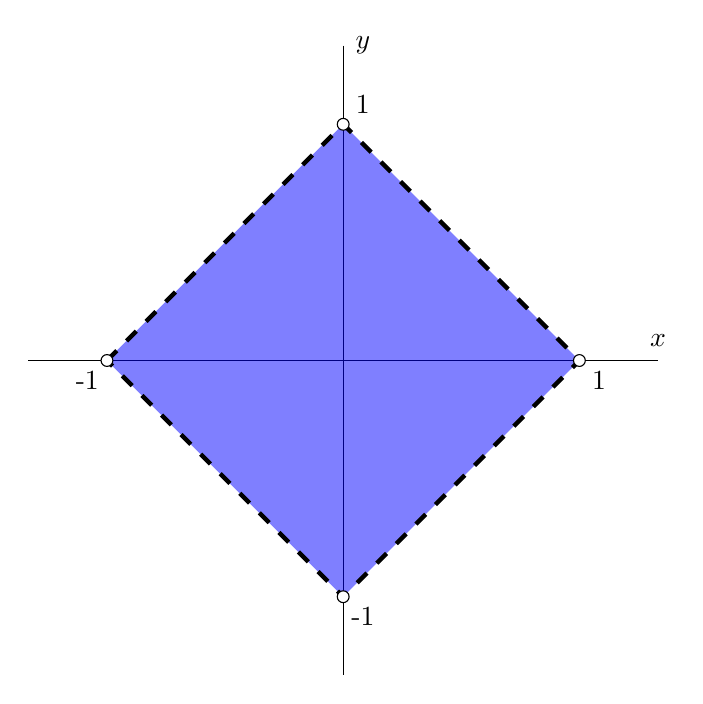
\begin{tikzpicture}
            \draw (-4,0) -- (4,0);
            \node at (4,0.25) {$x$};

            \draw (0,4) -- (0,-4);
            \node at (0.25,4) {$y$};

            \filldraw[ultra thick,dash=on 5pt off 5pt phase 10pt,fill=blue,fill opacity=0.5] (-3,0) -- (0,3) -- (3,0) -- (0,-3) -- cycle;

            \draw[fill=white] (-3,0) circle (0.075);
            \node at (-3.25,-0.25) {-1};

            \draw[fill=white] (3,0) circle (0.075);
            \node at (3.25,-0.25) {1};

            \draw[fill=white] (0,3) circle (0.075);
            \node at (0.25,3.25) {1};

            \draw[fill=white] (0,-3) circle (0.075);
            \node at (0.25,-3.25) {-1};
        \end{tikzpicture}
    \end{center}
    
Let $d_{std}$, $d_{l^\infty}$, and $d_{taxi}$ be shorthand for their respective metric spaces.

It is clear that each set is open in its respective metric space. Now consider the openness of each set in $d_{std}$. Since the open balls in $d_{l^\infty}$ and $d_{taxi}$ resemble open sets in standard Euclidian space, we know that they can be represented as a union of open balls, and thus are open in $d_{std}$.

Next, consider the openness of each set in $d_{l^\infty}$. We know that the open ball in $d_{l^\infty}$ is open in $d_{std}$, thus it can be represented by a union of open balls, thus any union of open balls in $d_{l^\infty}$ is also a union of open balls in $d_{std}$. Finally, since we know that the open balls in $d_{std}$ and $d_{taxi}$ are open in $d_{std}$, they can also be represented as a union of open balls in $d_{std}$, and thus as a union of open balls in $d_{l^\infty}$, thus each set is open in $d_{l^\infty}$.

A an argument similar to the above one shows that each set is also open in $d_{taxi}$.
    
\end{itemize}

\end{document}
